\section{Standard} 

% put the figure here for formatting reasons
\begin{figure*}[tb!]
    \centering
    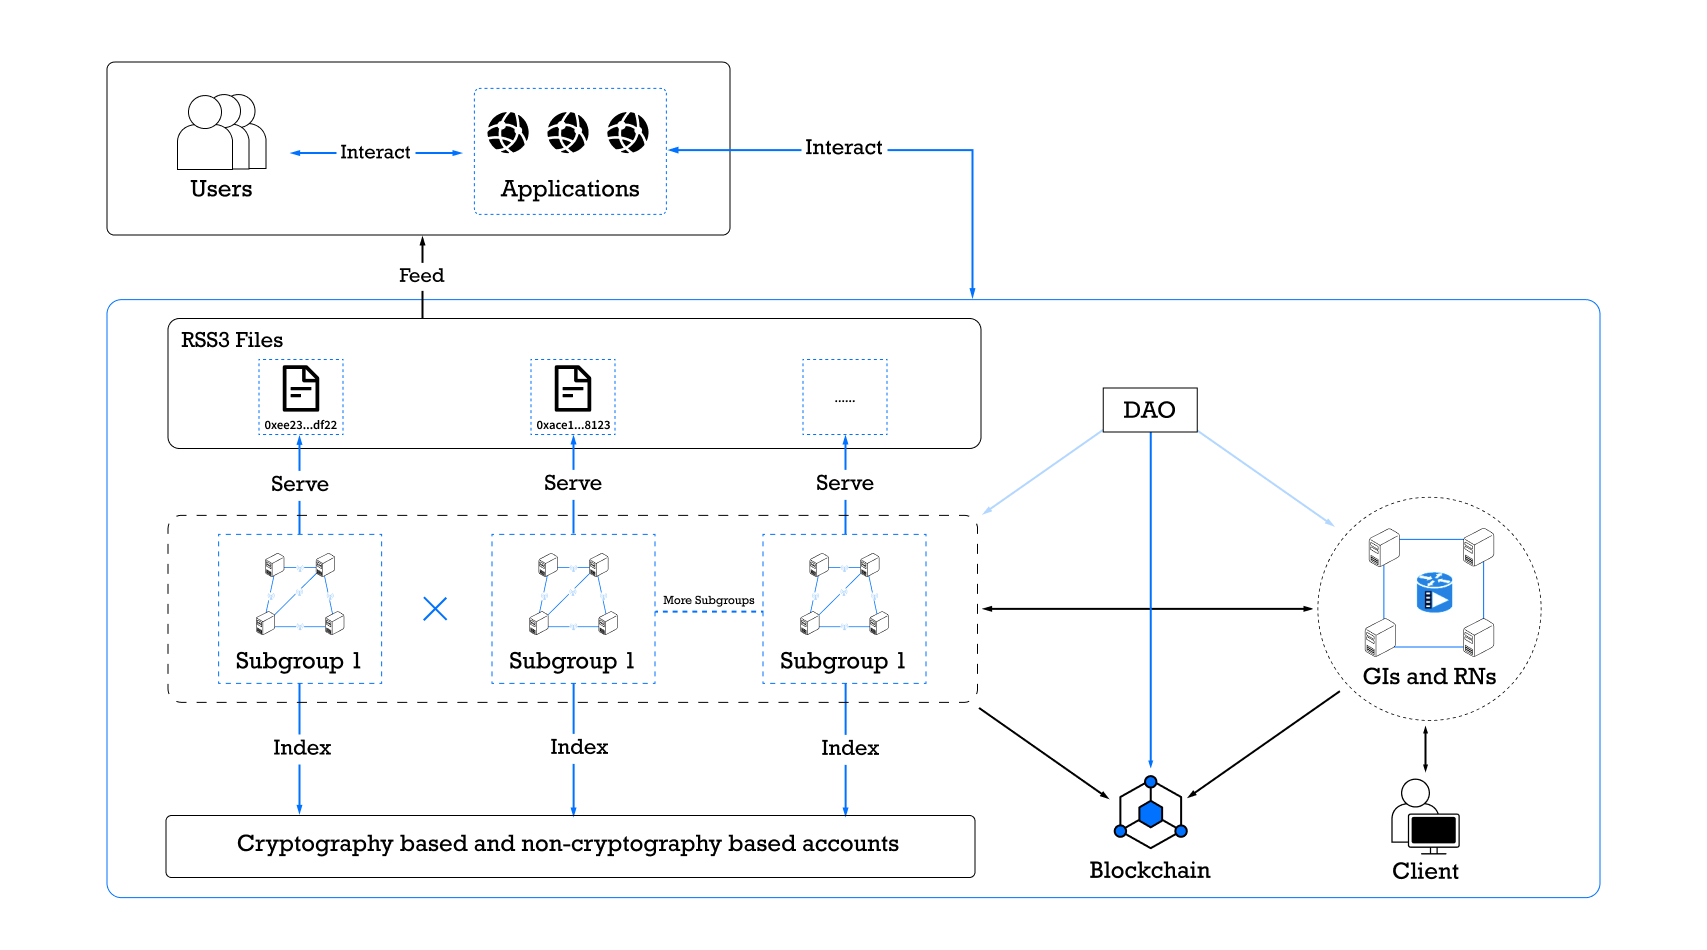
\includegraphics[height=9.3cm]{figures/network-arch.jpg}
    \caption{A typical RSS3 Network architecture.}
    \label{fig:network-arch}
\end{figure*}

Compared to its predecessor, RSS3 introduces fundamental changes to create an efficient and decentralized information distribution standard.

\subsection{Instance}

An instance is a collection of cryptography based accounts owned by one cyber existence. Upon registration, the first address submitted will be used as the instance's primary address. Additional accounts can be imported by auto-verification or user actions. All verified accounts will be stored in an RSS3 File. 

\subsection{Asset}

An asset refers to a medium of exchange owned by the instance that is digitally generated. An RSS3 network automatically incorporates instance assets from verified accounts, and stores them into the corresponding RSS3 File. DAO decides the rendering of assets in RSS3 Files as there are wide variations in types.

\subsection{Link}

Ubiquitous linking is the foundation of an open information system. The RSS3 Protocol supports universal links with customized types between RSS3 Objects. Major RSS3 Objects include:

\begin{itemize}
    \item Instance - a collection of cryptography based accounts
    \item Asset - a medium of exchange that is digitally generated
    \item Item - content generated on the network
\end{itemize}

An internal link is bidirectional which connects two objects within an RSS3 Network, whereas an external link unidirectionally connects an RSS3 Object with an external object. An external link destined for an RSS3 Object may be bidirectional if DAO approves the source.

\subsection{Governance and Ownership}

RSS3 network is equipped with a high Turing completeness. It is capable of handling sophisticated logic such as reviewing smart contracts that define permission and ownership of RSS3 Files.

\subsection{Activity Feed}

In an RSS3 File, an activity feed contains: 1) all activities indexed from the instance's verified accounts; 2) all items generated by the instance or the network; 3) all universal links generated on the RSS3 Network. The feed resembles the original RSS protocol with additional cryptographic information to support data integrity and originality. The design represents a decentralized approach for information distribution.

Based on the standard described above, we present the RSS3 Protocol, available at \url{https://github.com/NaturalSelectionLabs/RSS3}. The implementation is by no means a perfect solution to the problems which the web is facing now, but a significant leap forward toward a truly decentralized cyberspace.
